%!TEX root = ../main.tex

\section{Implementation} % (fold)
\label{sec:implementation}

Based upon the chosen design, a prototype will be developed. 
The prototype is separated into two parts: A visual representation of the weather data and an implementation of sonifications of the weather data. 



\subsection{Visual Implementation} % (fold)
\label{sub:visual_implementation}

As defined in the design chapter, visual representations of predefined weather data will be created.

The delimited weather data is:

\begin{itemize}
    \item Temperature - Current air temperature 2 meters above terrain.
    \begin{itemize}
        \item Day temperature
    \end{itemize}
    \item Wind speed - Average wind speed over 10 minutes, 10 meters above terrain.
    \item Pollen Forecast - The potency of the pollen.
    \item Visibility - How far can you see with clear line of sight.
    \item Downpour - Rain in mm.
\end{itemize}

Furthermore, the visual pretest(See section~\ref{sub:visual_pre_test}) has helped define which specific visualisations of weather data that are to be created( See table~\ref{tab:visual_pre_test}.
The results show the weather data along with descriptions of illustrations that should be implemented in each of the low, medium or high values of the different weather conditions.

Now that the visual pictures have been decided, the actual visualizations must be constructed.
The following visualization represents our interpretation of the visual test results(See Appendix~\ref{sub:processed_results}), and will be used as the visual representation of weather data in the actual test (See figure~\ref{fig:implementation11}).

\begin{figure}[!htbp]
    \centering
    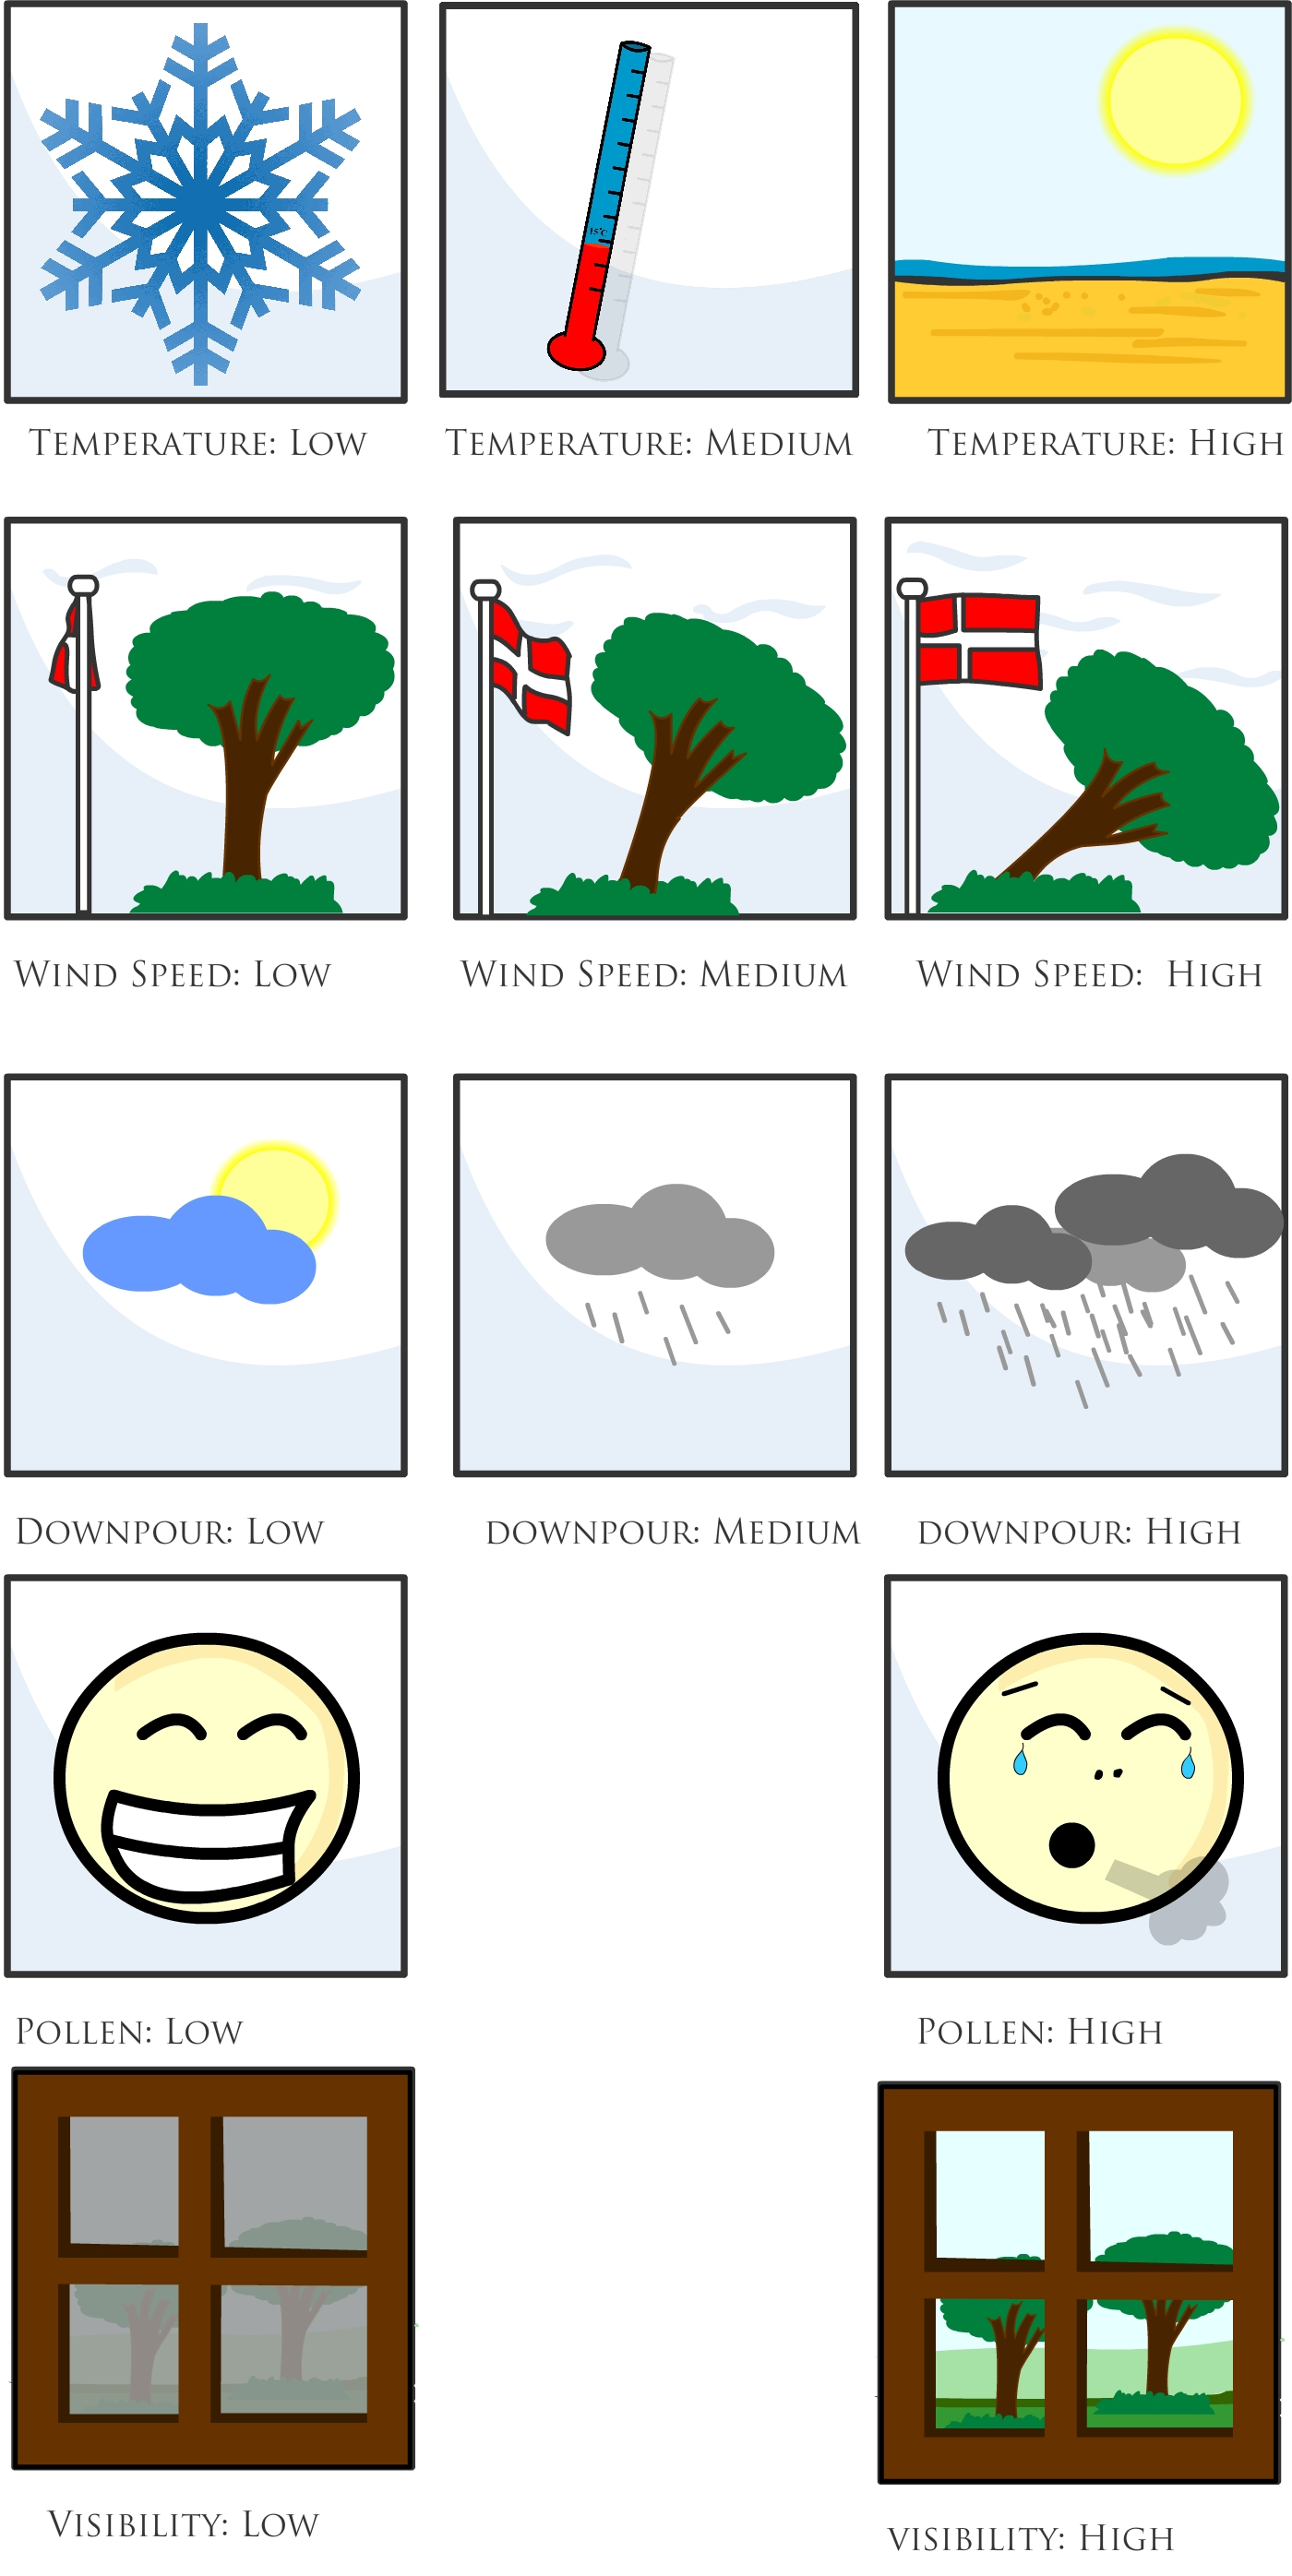
\includegraphics[width=0.7\textwidth]{images/Implementation11.jpg}
    \caption{Visual implementation}
    \label{fig:implementation11}
\end{figure}


% subsection visual_implementation (end)

\FloatBarrier
\subsection{Sound Implementation} % (fold)
\label{sub:sound_implementation}

As presented in the design (See section~\ref{ssub:how_the_sound_will_be_implemented_in_pure_data}), the following list is defined as the procedure of the implementation of the sounds in PureData.

\begin{enumerate}
    \item Input Sound
    \item Array / Sample
    \item Determine Sample Speed
    \item Phasor
    \item Merge Array and Sample Speed
    \item Fliter (if required)
    \item Output Sound
    \item Tracker
\end{enumerate}

Here is a overview of one of the pure data systems that has been made:

\begin{figure}[!htbp]
    \centering
    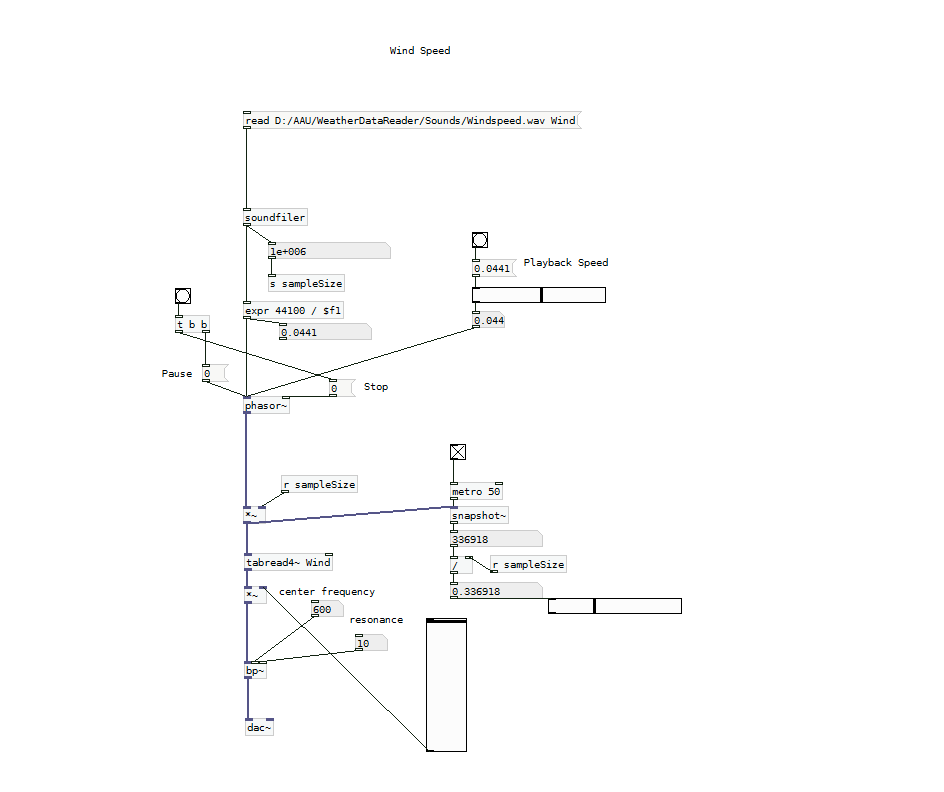
\includegraphics[width=1\textwidth]{images/Implementation1.png}
    \caption{Sample Pure Data implementation}
    \label{fig:implementation1}
\end{figure}

\FloatBarrier
\subsubsection*{Step 1} % (fold)
\label{ssub:step_1}

Here the program reads where the sound is placed on the computer and imports it into an array. 
As seen on the figure~\ref*{fig:implementation2} the path have been written down and in this case the array is called Wind.

\begin{figure}[!htbp]
    \centering
    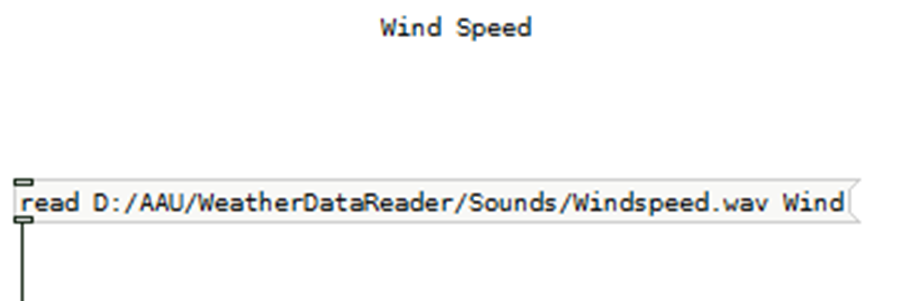
\includegraphics[width=.7\textwidth]{images/Implementation2.png}
    \caption{Sample audio import}
    \label{fig:implementation2}
\end{figure}

This is the array itself (Figure~\ref{fig:implementation3}). 
Here you can see what the different sound waves are going to look like. 
It might seem when you look at the arrays that there is a lot of wasted space in the array. 
This is simply because some of the sound don’t last that long and the empty space you see in the array is less than a second when played.

\begin{figure}[!htbp]
    \centering
    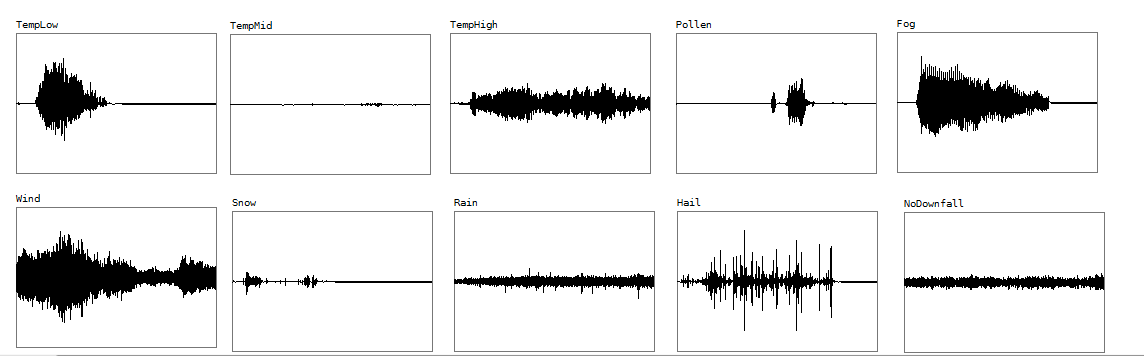
\includegraphics[width=.5\textwidth]{images/Implementation3.png}
    \caption{Sound sample array}
    \label{fig:implementation3}
\end{figure}

% subsubsection step_1 (end)

\FloatBarrier
\subsubsection*{Step 2} % (fold)
\label{ssub:step_2}

Here the soundfiler re-writes our floating points in the array to a binary sound file. 
As seen on the picture (Figure~\ref{fig:implementation4}) the sample amount is been read and stored in sampleSize which will be used later in the program to tell how big the array is. 
The samples then goes through a sampling that divides 44100 HZ with our sample size. This gives us the normal frequency. The data follows the path down to the phasor.

\begin{figure}[!htbp]
    \centering
    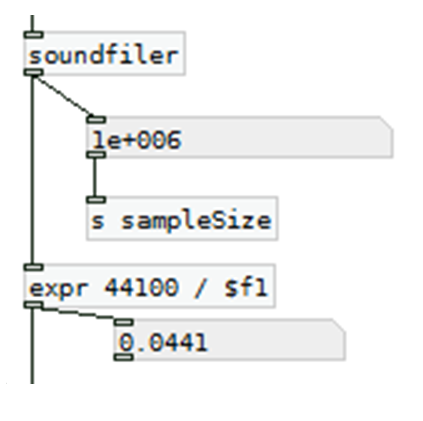
\includegraphics[width=.3\textwidth]{images/Implementation4.png}
    \caption{Soundfiler implementation}
    \label{fig:implementation4}
\end{figure}

% subsubsection step_2 (end)

\FloatBarrier
\subsubsection*{Step 3} % (fold)
\label{ssub:step_3}

We made a system that can control the speed of the samples. 
Using this, we can replace the original speed with our own to change the playback speed of the sound. 
This is using the custom made slider right besides the text Playback Speed on the picture (Figure~\ref{fig:implementation5}).

\begin{figure}[!htbp]
    \centering
    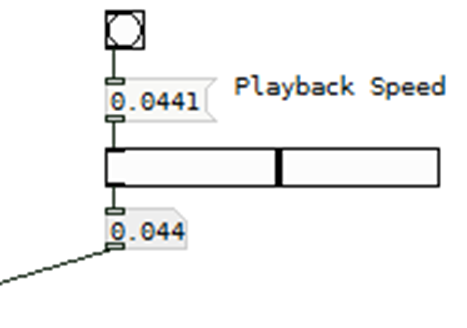
\includegraphics[width=0.3\textwidth]{images/Implementation5.png}
    \caption{Playback speep sample}
    \label{fig:implementation5}
\end{figure}

% subsubsection step_3 (end)

\FloatBarrier
\subsubsection*{Step 4} % (fold)
\label{ssub:step_4}

All the information sent to the phasor is now being used. The phasor detects a value between 1 and -1 to adjust the play speed. If the value is being set to 0 the waves in the phasor will be equal and stop the sound.
\begin{figure}[!htbp]
    \centering
    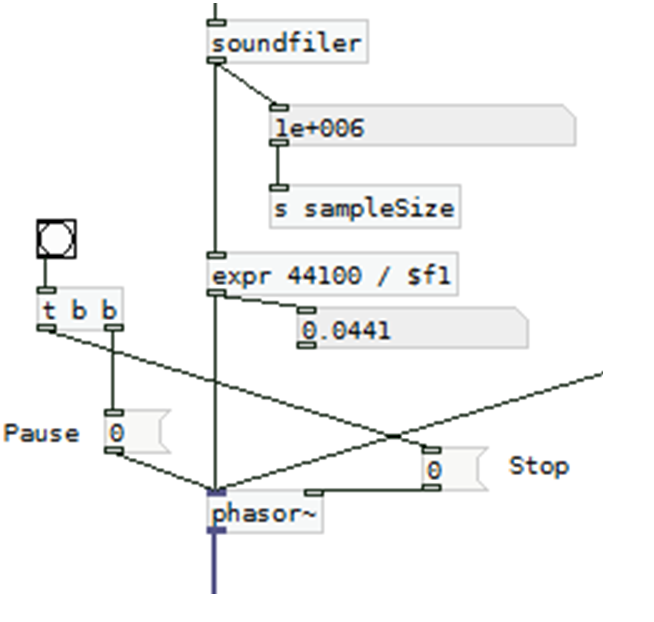
\includegraphics[width=0.3\textwidth]{images/Implementation6.png}
    \caption{Phasor}
    \label{fig:implementation6}
\end{figure}

% subsubsection step_4 (end)

\FloatBarrier
\subsubsection*{Step 5} % (fold)
\label{ssub:step_5}

Here (Figure~\ref{fig:implementation7}) 
The information from the phasor is being send into a binary signal operator that is being given a argument that is sampleSize. By doing this our progam now remembers how many samples there used to be. The samples can now merge with the array and tell what sample to move along further in the program.

\begin{figure}[!htbp]
    \centering
    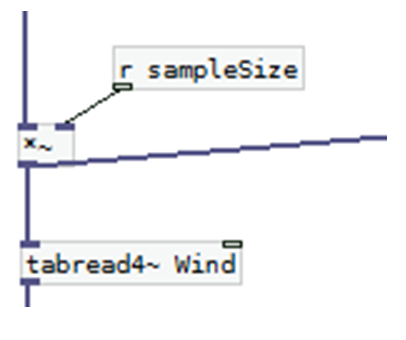
\includegraphics[width=0.3\textwidth]{images/Implementation7.png}
    \caption{Load old array}
    \label{fig:implementation7}
\end{figure}

% subsubsection step_5 (end)


\subsubsection*{Step 6} % (fold)
\label{ssub:step_6}

This is our bp filter as seen the two boxes linked to the filter are the center frequency and the resonance. 
In this case the center frequency is 600 and the resonance is 10.

\begin{figure}[!htbp]
    \centering
    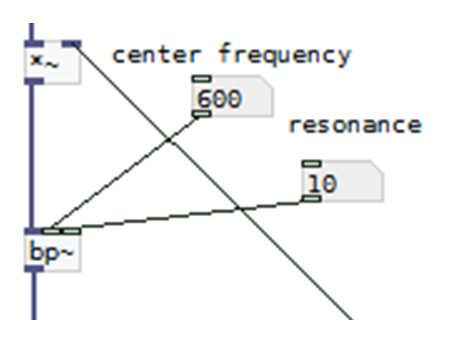
\includegraphics[width=0.3\textwidth]{images/Implementation8.png}
    \caption{bp Fliter}
    \label{fig:implementation8}
\end{figure}

% subsubsection step_6 (end)

\FloatBarrier
\subsubsection*{Step 7} % (fold)
\label{ssub:step_7}

After the filter all the information is sent to dac which is the audio output.

\begin{figure}[!htbp]
    \centering
    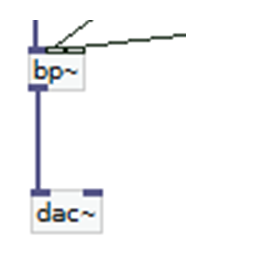
\includegraphics[width=0.2\textwidth]{images/Implementation9.png}
    \caption{dac output}
    \label{fig:implementation9}
\end{figure}

% subsubsection step_7 (end)

\FloatBarrier
\subsubsection*{Step 8} % (fold)
\label{ssub:step_8}

Additional feature:

A length tracker was implemented in order to know when the sound clip was done playing. This is done by tracking the samples going through the program.
This doesn’t change the sound output in any way but it’s useful to know during testing.

\begin{figure}[!htbp]
    \centering
    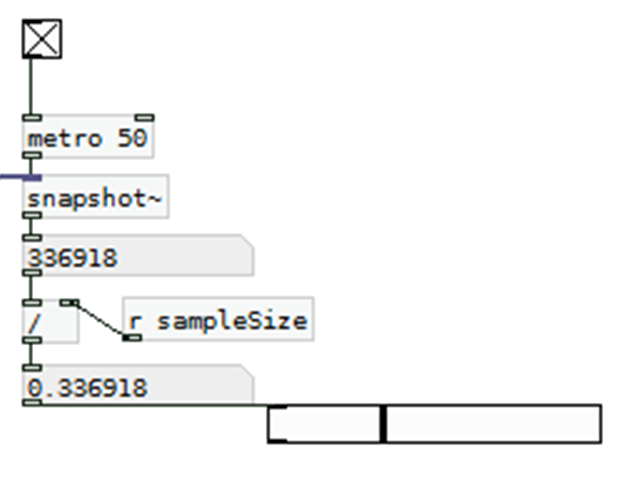
\includegraphics[width=0.3\textwidth]{images/Implementation10.png}
    \caption{Length Tracker}
    \label{fig:implementation10}
\end{figure}

\FloatBarrier
% subsubsection step_8 (end)

The rest of the sounds follow the same steps but the values is being replaced with these on our data sheet~\ref{tab:data_sheet}.

\begin{table}[!ht]
\centering
\begin{tabular}{l | l | l}
 & Play Speed & BP-Filter \\
\hline
Pollen & High: 0.418208 & N/A \\
\hline
Visibility & Low: 0.382 & N/A \\
\hline
Temperature & \specialcell{Low: 0.8339 \\ Mid: 0.0441 \\ High: 0.0882} & N/A \\
\hline
Downpour & \specialcell{Low: 0.06 \\ Mid: 0.2205 \\ High: 0.37} & N/A \\
\hline
Wind Speed & \specialcell{Low: 0.0441 \\ Mid: 0.0441 \\ High: 0.0441} & \specialcell{Low: 300 - 10 \\ Mid: 600 - 10 \\ high: 900 - 10}
\end{tabular}
\caption{Data sheet}
\label{tab:data_sheet}
\end{table}

Now that the sounds have been implemented the product is ready for testing. 
This leads us into the next step in the process, the evaluation of our prototype.
% subsection sound_implementation (end)

% section implementation (end)